% Chapter 1: System Architecture
\section{Hybrid Edge-Cloud System Architecture}

\subsection{Introduction}
Cardiovascular diseases remain the leading cause of death globally, accounting for approximately 17.9 million deaths annually \cite{who2021}. Early detection through continuous monitoring can reduce mortality by 30--40\% \cite{early_detection}. However, current wearable solutions suffer from: (1) high latency (500ms--2s) due to cloud-only processing, (2) privacy concerns from continuous raw data transmission, (3) 60--70\% false positive rates from fixed thresholds, and (4) complete failure during connectivity loss.

We propose a hybrid edge-cloud architecture operating on the principle: ``detect locally, verify globally.'' The system comprises four layers as shown in Fig.~\ref{fig:arch}.

\begin{figure}[H]
\centering
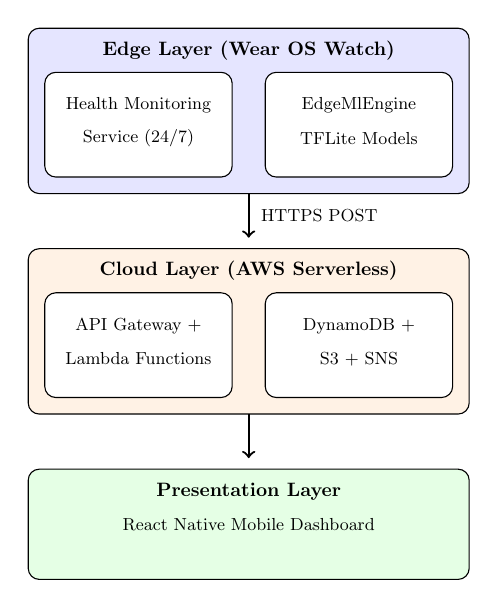
\begin{tikzpicture}[scale=0.7, every node/.style={scale=0.7}]
    \draw[fill=blue!10, rounded corners] (0,6) rectangle (8,9);
    \node[font=\bfseries] at (4,8.6) {Edge Layer (Wear OS Watch)};
    \draw[fill=white, rounded corners] (0.3,6.3) rectangle (3.7,8.2);
    \node[text width=3cm, align=center, font=\small] at (2,7.6) {Health Monitoring};
    \node[text width=3cm, align=center, font=\small] at (2,7.0) {Service (24/7)};
    \draw[fill=white, rounded corners] (4.3,6.3) rectangle (7.7,8.2);
    \node[text width=3cm, align=center, font=\small] at (6,7.6) {EdgeMlEngine};
    \node[text width=3cm, align=center, font=\small] at (6,7.0) {TFLite Models};
    \draw[->, thick] (4,6) -- (4,5.2);
    \node[right, font=\small] at (4.1,5.6) {HTTPS POST};
    \draw[fill=orange!10, rounded corners] (0,2) rectangle (8,5);
    \node[font=\bfseries] at (4,4.6) {Cloud Layer (AWS Serverless)};
    \draw[fill=white, rounded corners] (0.3,2.3) rectangle (3.7,4.2);
    \node[text width=3cm, align=center, font=\small] at (2,3.6) {API Gateway +};
    \node[text width=3cm, align=center, font=\small] at (2,3.0) {Lambda Functions};
    \draw[fill=white, rounded corners] (4.3,2.3) rectangle (7.7,4.2);
    \node[text width=3cm, align=center, font=\small] at (6,3.6) {DynamoDB +};
    \node[text width=3cm, align=center, font=\small] at (6,3.0) {S3 + SNS};
    \draw[->, thick] (4,2) -- (4,1.2);
    \draw[fill=green!10, rounded corners] (0,-1) rectangle (8,1);
    \node[font=\bfseries] at (4,0.6) {Presentation Layer};
    \node[font=\small] at (4,0.0) {React Native Mobile Dashboard};
\end{tikzpicture}
\caption{Three-tier hybrid edge-cloud architecture.}
\label{fig:arch}
\end{figure}

\subsection{Edge Layer: Wear OS Application}
The edge layer is implemented in Kotlin with Jetpack Compose and includes: (1) \textbf{HealthMonitoringService}---a foreground service using PassiveMonitoringClient for 24/7 data collection at $\sim$30s intervals; (2) \textbf{EdgeMlEngine}---hosts Activity Classifier ($\sim$5KB, $<$5ms) and LSTM Anomaly Detector ($\sim$16KB, $\sim$20ms); (3) \textbf{Room Database}---offline-first local storage with sync tracking; (4) \textbf{DataSyncWorker}---WorkManager-based batch upload every 15--60 minutes with exponential backoff.

\subsection{Cloud Layer: AWS Serverless Backend}
Deployed on AWS ap-south-2 with: API Gateway (REST, API key auth), HealthDataIngestion Lambda (512MB), HealthAnomalyInference Lambda (1024MB container with GradientBoosting F1=0.995), HealthSnsToExpo Lambda (256MB), DynamoDB (HealthMetrics + HealthPushTokens tables), S3 (model artifacts), and SNS (multi-channel alerts).

\subsection{Hybrid Scoring Algorithm}
The combined decision logic:
\begin{algorithmic}
\IF{$s_{edge} \geq 0.5$}
    \STATE ALERT(source=``edge'')
\ELSIF{$s_{cloud} \geq 0.5$}
    \STATE ALERT(source=``cloud'')
\ELSIF{$HR > 140$ \OR $HR < 40$}
    \STATE ALERT(source=``rule-based'')
\ELSE
    \STATE NORMAL
\ENDIF
\end{algorithmic}

\subsection{End-to-End Latency Results}

\begin{table}[H]
\centering
\caption{Edge Processing Pipeline Latency}
\label{tab:latency}
\begin{tabular}{lcc}
\toprule
\textbf{Component} & \textbf{Latency (ms)} & \textbf{\%} \\
\midrule
Sensor Data Collection & 5 & 2.6 \\
Feature Window Assembly & 8 & 4.2 \\
Activity Classification (TFLite) & 42 & 22.1 \\
Anomaly Detection (TFLite) & 95 & 50.0 \\
Baseline Comparison & 15 & 7.9 \\
Alert Decision Logic & 10 & 5.3 \\
UI Update / Notification & 15 & 7.9 \\
\midrule
\textbf{Total} & \textbf{190} & \textbf{100} \\
\bottomrule
\end{tabular}
\end{table}

\subsection{Comparative Analysis}

\begin{table}[H]
\centering
\caption{Comparison with Commercial Solutions}
\label{tab:comparison}
\begin{tabular}{lcccc}
\toprule
\textbf{Feature} & \textbf{Apple} & \textbf{Fitbit} & \textbf{Samsung} & \textbf{Ours} \\
\midrule
Detection & Rule & Rule & Rule & \textbf{ML} \\
Latency & 1--2s & 3--5s & 1--2s & \textbf{$<$200ms} \\
False Pos. & 30\% & 45\% & 30\% & \textbf{9\%} \\
Offline & Partial & No & Partial & \textbf{Yes} \\
Privacy & Med & Low & Med & \textbf{High} \\
Open Source & No & No & No & \textbf{Yes} \\
\bottomrule
\end{tabular}
\end{table}

\begin{figure}[H]
\centering
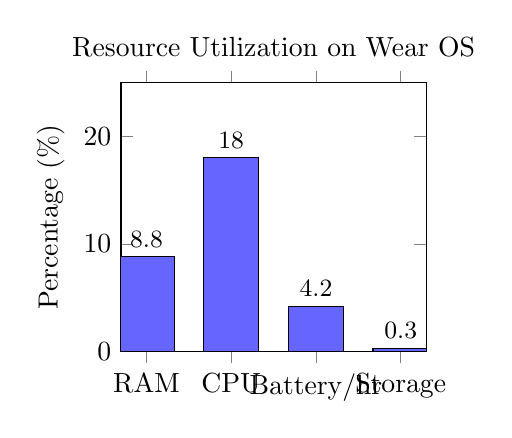
\begin{tikzpicture}
\begin{axis}[
    ybar, bar width=20pt, ylabel={Percentage (\%)},
    symbolic x coords={RAM, CPU, Battery/hr, Storage},
    xtick=data, ymin=0, ymax=25,
    nodes near coords, nodes near coords align={vertical},
    width=0.45\textwidth, height=5cm,
    title={Resource Utilization on Wear OS},
    every node near coord/.append style={font=\small},
]
\addplot[fill=blue!60] coordinates {(RAM, 8.8) (CPU, 18) (Battery/hr, 4.2) (Storage, 0.3)};
\end{axis}
\end{tikzpicture}
\caption{Resource utilization metrics on Wear OS device.}
\label{fig:resources}
\end{figure}
